\chapter{Introduction}
\label{ch:intro}

\section{Security Is Important, and Programming Languages Can Help!}

With the development of digital society, people are increasingly concerned about
the confidentiality of their personal data and the integrity of their online
assets. Increasingly relying on computing devices and the Internet in their
daily life, people fear that sensitive personal information, such as social
security numbers, medical records, bank account balances... may be revealed to
malicious third parties. People also worry that their digital photo albums,
signatures on online legal documents, spreadsheets in cloud storage... may be
tampered and manipulated by potential attackers.

Indeed, the fears are justified by recent news events. In 2018, the Cambridge
Analytica scandal hit the world headlines, where the data collected from 87
million social media users was misused without their consent
~\parencite{cadwalladr2018facebook,kitchgaessner2017cambridge,gonzalez2019global,hinds2020wouldn}.
In the healthcare sector, from 2005 to 2019, 249 million people were
affected by data breaches that caused exposure of sensitive medical
data~\parencite{seh2020healthcare}. Researchers have found ways to tamper with the
analytics APIs~\parencite{pfeffer2018tampering} and damage the integrity of
metadata, such as the numbers of likes, follows, and views, of major social
media platforms~\parencite{paquet2017can}. To deal with the security and privacy
challenges of the increasingly digitalized world, the European Union introduced
the General Data Protection Regulation (GDPR) to reform and regulate the
collection and processing of personal data. However, studies show that business
entities experience challenges in complying with GDPR or auditing for
compliance~\parencite{smirnova2024understanding}, particularly small-to-medium
size enterprises~\parencite{sirur2018we,freitas2018gdpr,harting2021impacts}.

\begin{figure}[tbp]
  \small
  \begin{align*}
    \langle \mathit{RECORD} \rangle ::= & {\color{green} \textbf{\{FirstName=}} \langle \mathit{ID} \rangle {\color{green} \textbf{;}} \\
                               & \enspace {\color{green} \textbf{LastName=}} \langle \mathit{ID} \rangle {\color{green} \textbf{;}} \\
                               & \enspace {\color{green} \textbf{SSN=}} \langle \mathit{SSN} \rangle {\color{green} \textbf{\}}} \\
    \langle \mathit{ID} \rangle     ::= & w , w \in \{ {\color{green} \textbf{A}}, ... {\color{green} \textbf{Z}}, {\color{green} \textbf{a}}, ... {\color{green} \textbf{z}} \}^{+} \\
    \langle \textit{SSN} \rangle    ::= & \langle D \rangle \langle D \rangle \langle D \rangle {\color{green} \textbf{-}}
                                 \langle D \rangle \langle D \rangle {\color{green} \textbf{-}}
                                 \langle D \rangle \langle D \rangle \langle D \rangle \langle D \rangle \\
    \langle D \rangle      ::= & d , d \in \{ {\color{red} \textbf{0}}, ... {\color{red} \textbf{9}} \}
  \end{align*}
  \caption{The user input grammar for a hypothetical application}
  \label{fig:grammar}
\end{figure}

From a technical perspective, ensuring the security and privacy of personal data
typically involves tracking and checking the flow of information. To ensure
confidentiality, data must not flow to inappropriate destinations, so that
sensitive personal information is not revealed; dually, to ensure integrity,
data must not flow from inappropriate sources, so that valuable digital assets
are not corrupted~\cite{sabelfeld2003language,biba1977integrity}. In practice,
such enforcement of the flow of information is often difficult to implement.
Take confidentially for example, software applications accept user input where
selected fields are sensitive, whose confidentiality is required during their
entire life cycle including both parsing and data processing. To rule out
information leaks, neither the sensitive fields, nor any data that depends on
those fields, is allowed to be revealed to a low-privilege observer. Consider a
web application that receives three fields from its user: (1) first name
(2) last name (3) social security number, the grammar of which
is defined in Figure~\ref{fig:grammar}, where terminals are divided into
low-security and high-security. The digits $d$ for social security number, being
confidential to users of the web application, are of high-security, so they are
marked {\color{red} red}, while other terminals, such as the keys of the record
and the strings $w$ for first name / last name, being safe to disclose, are all
of low-security, marked in {\color{green} green}. Consider the following user
input:

\begin{lstlisting}[numbers=none,xleftmargin=0.15\textwidth]
{FirstName=Mad;LastName=Hatter;SSN=012-34-5678}
\end{lstlisting}

\noindent It is tedious for the developer of this imaginary web application to track the
security level of data and check for information leaks. Software developers tend
to focus more on functionality in order to meet the tight software release
schedule and budget, thus software security usually only comes as an
afterthought
~\parencite{assal2018security,sharma2017aspects,steward2012software}.
Retrofitting security-related code often requires extensive modification to an
existing code-base and it relies on the programmers' skills and experience to
decide when and where such code should be placed. Furthermore, such modification
is error-prone: one single missing check could undermine the security of the
entire application.

\begin{figure*}[tbp]
  \small
  \center
\begin{tikzpicture}[scale=0.8]
\tikzset{level distance=50pt}
\Tree [
  .{ $\langle \mathit{RECORD} \rangle$ }
  {\color{green} \textbf{\{FirstName=}}
  [ .{ $\langle \mathit{ID} \rangle$ } {\color{green} \textbf{Mad}} ]
  {\color{green} \textbf{;LastName=}}
  [ .{ $\langle \mathit{ID} \rangle$ } {\color{green} \textbf{Hatter}} ]
  {\color{green} \textbf{;SSN=}}
                       [ .{ $\langle \mathit{SSN} \rangle$ }
                         [ .{ $\langle D \rangle$ } {\color{red} \textbf{0}} ]
                         [ .{ $\langle D \rangle$ } {\color{red} \textbf{1}} ]
                         [ .{ $\langle D \rangle$ } {\color{red} \textbf{2}} ]
                         {\color{green} \textbf{-}}
                                [ .{ $\langle D \rangle$ } {\color{red} \textbf{3}} ]
                                [ .{ $\langle D \rangle$ } {\color{red} \textbf{4}} ]
                                {\color{green} \textbf{-}}
                                       [ .{ $\langle D \rangle$ } {\color{red} \textbf{5}} ]
                                       [ .{ $\langle D \rangle$ } {\color{red} \textbf{6}} ]
                                       [ .{ $\langle D \rangle$ } {\color{red} \textbf{7}} ]
                                       [ .{ $\langle D \rangle$ } {\color{red} \textbf{8}} ] ]
                       {\color{green} \textbf{\}}}
]
\end{tikzpicture}
\caption{The parse tree generated from the example user input.
  All terminals are represented as labeled values:
  the {\color{red} red} ones, such as the digits of SSN,
  are of high-security, while the {\color{green} green} ones, such as the keys
  of the record and first name / last name, are of low-security.}
\label{fig:parsetree}
\end{figure*}

Alternatively, the author of the web application could implement a parser for
the grammar in Figure~\ref{fig:grammar} in a programming language that enforces
information-flow security. Each terminal in the grammar would be labeled with a
security level and the programming language, instead of some ad-hoc checks
implemented by the programmer of the web application, would guarantee that the
high-security information is only present in those parts of the output parse
tree that are marked as high-security. For example, according to the grammar in
Figure~\ref{fig:grammar}, the example user input string is parsed into the parse
tree in Figure~\ref{fig:parsetree}, where the terminal nodes that represent
digits of the social security number are of {\color{red} high-security}, while
the terminals that compose the rest of the input string are of {\color{green}
  low-security}. The confidentiality of SSN is guaranteed during data processing
by the programming language itself. When the web application interacts with the
outside world, such as making a foreign function interface (FFI) call or storing
into a database, the conceptual language should encrypt whatever values labeled
as high security before they are passed into a foreign routine. The programming
language-based approach of information-flow
security~\parencite{sabelfeld2003language} alleviates the security burden of
software development, because it forms an abstraction over the flows of
information and decouples security from the functionality of a software
application.


\section{Information-Flow Control via Static, Dynamic, and Hybrid Mechanisms}

%% \todo[inline]{Let's have some examples in this chapter -Jeremy}

Information-flow control (IFC) ensures that information transfers within a
program adhere to a security policy, for example, by preventing high-security
data from flowing to a low-security channel. This adherence can be enforced
statically using a type
system~\parencite{volpano1996sound,Myers:1997aa,myers1999jflow}, or dynamically
using runtime
monitoring~\parencite{Askarov:2009vq,austin2009efficient,Devriese:2010up,stefan2011flexible,Austin:2017uh,Xiang:2021ub},
or using static analysis to pre-compute information that facilitates runtime
monitoring
~\parencite{le2005monitoring,le2007automaton,Chandra:2007we,Shroff:2007tg,russo2010dynamic,moore2011static}.
The static and dynamic approaches have complementary strengths and weaknesses;
the dynamic approach requires less effort from the programmer while the static
approach provides stronger guarantees and less runtime overhead. The main
theorem of an IFC system is \textit{noninterference}~\cite{goguen1982security}.
Informally, noninterference states that, if the secretive user input varies, the
public output of the program must stay the same.

%% \todo[inline]{add another sentence that explicitly road-maps the rest of this
%%   section. -Jeremy}
We are going to review the literature about static and dynamic enforcement of
IFC in Section~\ref{sec:intro-static-ifc} and Section~\ref{sec:intro-dyn-ifc}
respectively. We then review dynamic IFC enforcement with static pre-processing
in Section~\ref{sec:intro-dyn-static}. Finally in
Section~\ref{sec:intro-hybrid}, we briefly review the hybrid technique
by~\textcite{Buiras:2015aa}, which offers the programmer control over the
regions where IFC is enforced statically versus dynamically in a single program.

\subsection{Static IFC in Programming Languages}
\label{sec:intro-static-ifc}

The interest in enforcing confidentiality and regulating the flow of information
in a computer program arose with applications to defense in the 1970s
\autocite{bell1976secure}. \textcite{denning1976lattice} builds an information
flow model using a lattice of security labels and
\textcite{denning1977certification} describe a static analysis for information
flow, with a proof that a certified program will not transmit confidential input
to non-confidential output. They distinguish between two types of information
flows: explicit flow and implicit flow. Consider the assignment \texttt{x := y +
  z}, there are explicit flows from \key{y} to \key{x} and from \key{z} to
\key{x}, because both \key{y} and \key{z} affect the value that \key{x} is
assigned to. The certification checks whether the join (least upper bound) of
the security of \key{y} and {z} is less than or equal to the security of
\key{x}. Implicit flows, on the other hand, arise from the branching structure
of a program. Consider the program \texttt{if x then y := y + 1 else ()}. An
observer is able to learn whether \key{x} is true or false, by inspecting
whether \key{y} increments. To control the implicit flow, the certification
checks whether the security of \key{x} is less than or equal to that of \key{y}.
%% \todo[inline]{What are the main ideas for how this static analysis works? -Jeremy}

\textcite{volpano1996sound} further develop the static enforcement and propose a
typed-based approach to IFC, by defining a type system for an imperative
programming language and proving its security with a type soundness proof. The
type system approach benefits IFC enforcement because it is compositional: the
security of the entire program is determined from the security of its
constituent components; secure components form a larger secure system as long as
their type signatures agree~\cite{sabelfeld2003language}. By writing a program
that type checks, the software developer constructs a proof that the program is
indeed secure.
%% \todo[inline]{What are the important differences in the
%%   type-based approach? Is it the compositionality? If so, say that right away.
%%   -Jeremy}
%% \todo[inline]{Give the technical definition of compositional.}

We explain how a type system defends against illegal information flow using
examples. Consider two IO functions: \texttt{private-input} and
\texttt{publish}: the former returns a high-security boolean that represents
sensitive user input information; the latter takes a low-security boolean and
publishes it into a publicly visible channel.

\paragraph{Explicit flow} Consider the program with an illegal explicit flow
from private input to public output:
\begin{verbatim}
  let input = private-input () in publish (¬ input)
\end{verbatim}
The program is rejected by the type checker, because \texttt{(¬ input)} is typed
at $\Bool_{\high}$ but \texttt{publish} expects its argument to be of
$\Bool_{\low}$, $\high \npreccurlyeq \low$. As a result, the type system
prevents information from leaking through explicit flow. On the other hand, the
program
\begin{verbatim}
  let input = private-input () in publish (¬ true)
\end{verbatim}
is accepted by the type checker, because \texttt{(¬ true)} is typed at
$\Bool_{\low}$, which can flow into \texttt{publish}. Indeed, the output remains
constant regardless of user input, so no information leaks through the output.

\paragraph{Implicit flow} Guarding against illegal implicit flows is
more involved: the type system estimates the security of an if-conditional by
joining the security of its branches with that of the branch condition (often
referred to as type stamping). Consider the following program with an illegal
information flow from private input to public output:
\begin{verbatim}
  let input = private-input () in
    publish (if input then false else true)
\end{verbatim}
The input influences the output through the branching structure of the program:
if input is true, the then-branch is taken and the output is false; if input is
false, the else-branch is taken and the output is true. The branch condition is
typed at $\Bool_{\high}$ and the branches are typed at $\Bool_{\low}$, so the
entire \texttt{if} has type $\Bool_{\low \curlyvee \high} = \Bool_{\high}$.
Again, \texttt{publish} expects $\Bool_{\low}$, so the program is rejected.
Consequently, the type system guards against the information leak through
implicit flow.

\textcite{heintze1998slam} and~\textcite{zdancewic2002programming} further
develop the type system approach to IFC and add support for higher-order
functions. Researchers also build IFC type systems for bytecode intermediate
languages \autocite{barthe2005non}, for object-oriented languages
\autocite{amtoft2006logic}, and for reactive programming languages
\autocite{bohannon2009reactive}. Although the aforementioned languages are
mostly theoretical, efforts have also been made to integrate information flow
control into off-the-shelf programming languages, such as Jif for Java
\autocite{myers1999jflow} and Flow Caml for OCaml
\autocite{pottier2002information, simonet2003flow}.

\subsection{Dynamic IFC in Programming Languages}
\label{sec:intro-dyn-ifc}

%% \todo[inline]{The above is for pure (no
%%   mutation) languages. -Jeremy}
%% \todo[inline]{What exactly is the dynamic
%%   checking doing? -Jeremy }
%% \todo[inline]{The NSU stuff is for languages with
%%   mutation. -Jeremy}
%% \todo[inline]{What's coarse-grained IFC? What's floating
%%   label? -Jeremy}

IFC can also be enforced dynamically using runtime monitoring. Values typically
have security labels associated with them and the runtime monitor tracks those
labels during program execution. In the illegal explicit flow example
\begin{verbatim}
  let input = private-input () in publish (¬ true)
\end{verbatim}
the value of \texttt{input} is tagged with \high and so is its negation. When
\texttt{publish} is called, the function checks whether the label on the
argument is \low. The check fails, so the monitor reports a runtime error. In
the constant example
\begin{verbatim}
  let input = private-input () in publish (¬ true)
\end{verbatim}
\texttt{true} is tagged with \low and so is its negation; the monitor succeeds
and publishes \texttt{false}. In the illegal implicit flow example
\begin{verbatim}
  let input = private-input () in
    publish (if input then false else true)
\end{verbatim}
the label associated with the evaluation result of the if-conditional is the
join between that of the branch taken and that of the branch condition; in this
case, $\low \curlyvee \high = \high$. The \texttt{publish} function again checks
the label against \low, $\high \npreccurlyeq \low$, so it results in a runtime
error.

\textcite{li2006encoding,LI20101974} study dynamic IFC for purely functional
languages (no mutable states). They add dynamic checking of information flow
control to Haskell, by utilizing existing language features, specifically arrows
and typeclasses.

\textcite{austin2009efficient} consider IFC for Javascript, a language with
mutable references. They propose a dynamic approach called
\textit{no-sensitive-upgrade} (NSU) checking, which guards against illegal
implicit flows through the heap. During execution, the language runtime keeps
track of a special security label, namely program counter. The program counter
starts from low and is updated to high when the program branches on a
high-security value. NSU terminates the execution whenever the program attempts
to modify a low-security memory location under a high-security program counter.
%% \todo[inline]{need to explain ``high-security context''}
\textcite{austin2010permissive} study a sound yet more flexible enforcement
strategy called \textit{permissive-upgrade}. Compared to NSU, permissive-upgrade
allows more programs to run to completion.
\textcite{austin2012multiple,Austin:2017uh} propose \textit{faceted values},
another approach to dynamically handle implicit flows by simulating
multi-execution in a single process, which, unlike no-sensitive-upgrade and
permissive-upgrade, avoids conservative monitor failures.

\textcite{stefan2011flexible,stefan2012flexible,STEFAN:2017ta} design a Haskell
library called LIO. LIO is implemented as a domain specific language (DSL)
embedded in Haskell. Even though Haskell itself is purely functional, it is
worth noting that the LIO DSL does support mutable references (\key{LIORef}).
Inspired by IFC operating systems
~\parencite{efstathopoulos2005labels,zeldovich2011making,krohn2007information,vandebogart2007labels},
LIO makes two unique design choices: (1) coarse-grained labeling (2) a floating
current label. LIO is ``coarse-grained'' in that not all values are labeled by
default. A programmer need to use the \key{toLabeled} primitive to explicitly
protect a value. In this way, a programmer may choose to label a value when it
is necessary to impose flow control policies and omit the labels for
security-insensitive parts of the program. In LIO, the ``current label'' serves
as a security upper bound of all values. During program execution, the LIO
runtime raises the current label to ``float'' above the security of all data
read by the current computation. Similar to NSU, LIO performs dynamic checking
on heap write operations and disallows writing to memory locations whose
security is below the current label. Under the hood, LIO keeps track of the
current label as a monad.

\subsection{Dynamic IFC Augmented With Static Pre-processing}
\label{sec:intro-dyn-static}

Researchers have also explored facilitating runtime IFC monitors with static
analyses prior to program execution, to achieves goals that are hard to
accomplish by using dynamic IFC alone. It is worth noting that different from
user-controlled hybrid IFC and gradual IFC (which we are going to discuss in
Section~\ref{sec:intro-hybrid} and Section~\ref{sec:intro-gradual-ifc}
respectively), papers in this category do not aim at offering programmer the
\emph{control} over statically versus dynamically enforced regions in a single
program.

\textcite{le2005monitoring} explore a
hybrid IFC monitor for sequential programs that combines runtime IFC with a
static analysis that gathers information about the non-executed branches. This
hybrid IFC accepts programs that are conservatively rejected by fully static
IFC. They further show that it is possible to alter the behavior of executions
that may be unsafe by resetting output values using the information from their
hybrid analysis to reclaim confidentiality. \textcite{le2007automaton} extends
this hybrid IFC approach to concurrent programs and prove noninterference for
any execution. \textcite{Shroff:2007tg} build a runtime monitor augmented with a
pre-computed fixed point of dependencies. Similar to
\textcite{le2005monitoring}, they observe that this hybrid technique is less
conservatively than a fully static system. They also show that their hybrid
monitor is able to support user-defined policy, so that different policies can
be applied to the same program.

\textcite{Chandra:2007we} implement a hybrid monitor for the Java virtual
machine. Their implementation add IFC annotations to a executable file using a
static analysis. The runtime monitor then uses those annotations to update the
labels of variables in alternative execution paths to enforce IFC, while
maintaining backward-compatibility with existing Java class files.

\textcite{russo2010dynamic} study dynamic IFC in a flow-sensitive setting. They
utilize a static analysis that detects variables in untaken branches whose
security must be upgraded at runtime in order to prevent illegal implicit flows
through the heap. \textcite{moore2011static} improve the efficiency of the
hybrid monitoring of \textcite{russo2010dynamic} by selectively tracking
variables and incorporating memory abstractions.

\subsection{Programmer-Controlled Hybrid IFC}
\label{sec:intro-hybrid}

Similar to gradual IFC and different from dynamic IFC with static
pre-processing, Hybrid LIO (HLIO)~\cite{Buiras:2015aa} supports programmer's
choice of static or dynamic IFC in different regions of a single program. By
default, the checking is static, but a programmer can insert a \texttt{defer}
clause to say that the security constraints should be checked at runtime. There
are two major differences between HLIO and gradual IFC programming languages (we
are going to discuss gradual IFC in the next section). In HLIO, the developer
has to embed explicit \texttt{defer} into the program, while in a gradual
language, the switch between static and dynamic is directed by types, with no
\texttt{defer} or explicit casts needed. Moreover, there is no theorem about
adding and removing \texttt{defer} in HLIO, while in a gradual language, the
gradual guarantee theorem relates the runtime behavior of programs that differ
only in the precision of their type annotations.

\section{The Tension Between Gradual Typing and Information-Flow Control}
\label{sec:intro-gradual-ifc}

Taking inspiration from gradual typing~\parencite{Siek:2006bh,Siek:2007qy},
researchers have explored new ways to give programmers control over which parts
of the program are secured statically versus dynamically, directed by
\textit{type annotations}. In general, gradually typed languages support the
seamless transition between static and dynamic enforcement through the
\textit{precision} of type annotations. Gradual security is useful, because the
programmer is free to choose when it is appropriate to increase the precision of
the type annotations and put in the effort to pass the static checks and when it
is appropriate to reduce the precision of type annotations, deferring the
enforcement to runtime.

The main challenge in the design of gradually typed languages is controlling the
flow of values (and information) between the static and dynamic regions of code,
which is accomplished using runtime casts. Typically source programs are
compiled to an intermediate language, called a cast calculus, that includes
explicit syntax for runtime casts. \textcite{Disney:2011fv} design a cast
calculus with IFC for a pure lambda calculus and prove noninterference.
\textcite{Fennell:2013ab} design a cast calculus named ML-GS with mutable
references using the no-sensitive-upgrade (NSU) runtime checks of
\textcite{austin2009efficient}. \textcite{Fennell:2015aa} design a cast calculus
for an imperative, object-oriented language.

\begin{table}[tbp]
  \footnotesize
  \centering
  \caption{Proposed sources of tension between security and the gradual guarantee}
  \begin{tabularx}{\textwidth}{X|c|c|c|c|c}
  \toprule
  \thead{Language} & \thead{Security \\ (noninterference)} & \thead{Gradual\\Guarantee} &
  \thead{Type-guided \\ classification} & \thead{NSU \\ checking} & \thead{Runtime \\ security labels} \\
  \hline
  \GSLRef    & \tikzmark{a}{\yes}  & \cellcolor{Red!10} \tikzmark{b}{\no} & \yes  & \yes & $\{ \low, \high, \unk \}$ \\[1ex]
  \hline
  GLIO      & \yes & \cellcolor{Green!10} \tikzmark{c}{\yes} & \tikzmark{d}{\no}  & \yes & $\{ \low, \high \}$ \\[1ex]
  \hline
  \WHILEG & \yes & \cellcolor{Green!10} \tikzmark{e}{\yes} & \yes   & \tikzmark{f}{\no} & $\{ \low, \high, \unk \}$ \\[1ex]
  \hline
  \rowcolor{highlight}
  \Surface~{\scriptsize (this dissertation)} & \yes & \cellcolor{Green!10} \tikzmark{g}{\yes} & \yes & \yes & \tikzmark{h}{$\{ \low, \high \}$} \\[1ex]
  \bottomrule
  \end{tabularx}
\begin{tikzpicture}[overlay, remember picture, yshift=.25\baselineskip, shorten >=.5pt, shorten <=.5pt]
  \draw[dashed,thick] (a) to [bend right=15] (b);
  \draw[dashed,thick] (c) to [bend right=15] (d);
  \draw[dashed,thick] (e) to [bend right=10] (f);
  \draw[thick]        (g) to [bend right=8 ] (h);
\end{tikzpicture}
  \label{tab:cc-features}
\end{table}

The main property of gradually typed languages is the \textit{gradual
  guarantee}~\cite{Siek:2015ac}, which states that removing type annotations
should not change the runtime behavior. Adding type annotations should also
result in the same behavior except that it may introduce more trapped errors
because those new type annotations may contain mistakes. Since the formulation
of the gradual guarantee as a criterion for gradually typed
languages~\cite{Siek:2015ac}, researchers have explored the feasibility of
satisfying both the gradual guarantee and noninterference.
\textcite{Toro:2018aa} identify a tension between the gradual guarantee and
security enforcement. They analyze the semantics of runtime casts through the
lens of Abstracting Gradual Typing~\parencite{Garcia:2016aa} and propose a
type-driven semantics for gradual security. However, \textcite{Toro:2018aa}
discover counterexamples to the gradual guarantee in the \GSLRef language. They
conjecture that it is not possible to enforce noninterference and satisfy the
gradual guarantee at the same time.

\textcite{Amorim:2020aa} conjecture one possible source of the tension: the
\textit{type-guided classification} performed in
\GSLRef~\parencite{Toro:2018aa}. They propose a new gradually typed language,
GLIO, which sacrifices type-guided classification. They prove that GLIO
satisfies both noninterference and the gradual guarantee using a denotational
semantics.
%
\textcite{bichhawat2021gradual} conjecture that \textit{NSU checking} could be
another possible source of the tension. As an alternative, they propose a hybrid
approach that leverages static analysis ahead of program execution to determine
the write effects in untaken branches. They study a simple imperative language
with first-order stores and prove both noninterference and the gradual
guarantee.

A ideal gradual IFC language (1) should enforce security by
satisfying noninterference (2) should satisfy the gradual guarantee (3) should
provide type-based reasoning through vigilance and type-guided classification
(4) should not require addition static analyses prior to program execution.
Contrary to the prior work, I am going to show in this dissertation that one
does not have to give up on any of the four requirements to resolve the tension
between noninterference and the gradual guarantee. Instead, the real source of
the tension is that \GSLRef allows \unk as a \emph{runtime} security label. By
walking back this usual design choice, I am going to present a gradual
IFC programming language \Surface and prove that \Surface satisfies
both noninterference and the gradual guarantee without any sacrifices.

\section{Key Enabling Insight}

In \GSLRef{}, one can write a literal such as $\true_{\unk}$ in a program. At
runtime, the literal becomes a value of unknown security level. I observe that
allowing \unk as a \emph{runtime} security label is the main reason that \GSLRef
violates the gradual guarantee. That design of \GSLRef was unusual because the
unknown type $\unk$ is traditionally used in gradual languages to represent the
lack of static information, not the lack of dynamic information. The design is
also unusual when compared to dynamic systems for IFC, as those systems do not
use an unknown security
level~\parencite{Askarov:2009vq,austin2009efficient,Devriese:2010up,stefan2011flexible,Austin:2017uh}.

Based on this observation, I propose a new gradual, IFC language \Surface, which
(1) enforces information flow security, (2) satisfies the gradual guarantee, (3)
enjoys type-based reasoning through free theorems, and (4) utilizes NSU checking
to enforce implicit flows through the heap with no static analysis required. In
\Surface, runtime security labels do not include \unk, only \low and \high (or
any lattice of security labels). On the other hand, to support gradual typing,
the security labels in a type annotation may include \unk. Surprisingly, I
discover that removing \unk from the runtime labels is sufficient to reclaim the
gradual guarantee, without sacrificing type-guided classification as in GLIO or
NSU checking as in \WHILEG. This finding is the primary contribution of this
dissertation. In \Surface, the security level of a literal defaults to \low,
similar to systems like Jif~\parencite{Myers:2006aa} and GLIO, but different
from \GSLRef and \WHILEG.

One might think that allowing $\unk$ as a label on literals and therefore on
values is necessary so that programmers can run legacy code (without any
security annotations) in a gradual language, by making \unk the default label
for literals. However, prior information-flow languages use \low security as the
default security label for literals~\parencite{Myers:2006aa} and for good
reasons. The security of a literal is something that only the programmer can
know. That is, the identification of high-security data in a program must be
considered as an input to an information flow system, and not something that can
or should be inferred. When migrating legacy code into a system that supports
secure information flow, a necessary part of the process for the programmer is
to identify whether there is any high-security information in the legacy code.
The choice of \low as the default label is because most literals (if not all) in
real programs are low security. In fact, it is bad practice to embed
high-security literals, such as passwords, in program text.

\section{Thesis Statement}

{\color{NavyBlue} %%% new text
The main enabling insight leads us to the thesis of this dissertation. My thesis
is that a gradual IFC programming language is able to satisfy the gradual
guarantee while supporting type-based reasoning, as long as there is no \unk
among runtime security labels, and the language uses security coercions as the
representation for casts:

\vspace{20pt}
\fbox{
	\parbox{0.9\linewidth}{\textbf{\Large \ul{My thesis:}\\ It is possible to
      design a gradual IFC programming language that satisfies both
      noninterference and the gradual guarantee while supporting type-based
      reasoning, by excluding the unknown label \unk from runtime security
      labels and using security coercions to represent casts.}
  }
}
}%%% end new text

\section{Technical Contributions and Outline}

The semantics of \Surface is given by translation to a new security cast
calculus \CC. I first define a syntax, type system, and operational semantics
for \CC. I then compile \Surface into \CC in a type-preserving way.

In \CC, \textit{security coercions} serve as the runtime security monitor, in
which I adapt ideas from the Coercion
Calculus~\parencite{Henglein:1994nz,Herman:2010aa} to IFC. A coercions on
security labels can be an \textit{injection} from a security label to \unk or a
\textit{projection} from \unk to a security label. Security labels on literals
in \Surface become the sources of injections in \CC, while runtime NSU checks
are treated as a special kind of projection where the target is the security
level of the memory location to modify. Information flow policies are enforced
when security coercions are reduced to their normal forms. \textit{Composing}
coercions models \textit{explicit flows}, while the action of \textit{stamping}
a coercion in normal form models \textit{implicit flows}.

Compared to prior work on gradual IFC languages, the \CC cast calculus supports
an additional feature called \textit{blame tracking}~\parencite{Findler:2002eu}.
Blame tracking is important because it enables modular runtime error messages,
for example, they play an important role in production-quality languages such as
Typed Racket~\parencite{Tobin-Hochstadt:2008lr,Preston-Tunnell-Wilson:2018aa}.

Compared to prior work on gradual IFC based on abstracting gradual typing
(AGT)~\parencite{Toro:2018aa}, my use of a cast calculus makes it clear where
in the program there is runtime overhead from dynamic checking (the casts). This
is important for the programmer to know because one may wish to avoid runtime
overhead in hot regions of a programs. In the translation from \Surface to \CC,
casts are only inserted where there is insufficient information during
compilation to decide whether a security policy is enforced or not. In
particular, casts are not inserted in statically typed regions. In this way,
information flows that are statically ensured to be safe will never be checked
again at runtime. On the contrary, the AGT mechanism for dynamic checking
(called evidence) is attached to most nodes in the syntax tree.

{\color{NavyBlue} %%% new text
In summary, my dissertation makes the following technical contributions:

\begin{enumerate}
\item Identify the main cause of the tension between information flow security
  and the gradual guarantee in \GSLRef: the inclusion of \unk in the runtime
  security labels.
\item Two coercion calculi that serve as the runtime IFC monitor: a coercion
  calculus for security labels and a coercion calculus for secure values.
\item A cast calculus \CC with IFC that defines the dynamic semantics of
  \Surface.
\item The Agda formalization of \Surface and its cast calculus \CC.
\item A proof of noninterference for \Surface through the simulation between its
  cast calculus \CC and a dynamic IFC programming language \DynIFC.
\item \Surface, the first gradual IFC language with type-guided
  classification that satisfies the gradual guarantee.
\end{enumerate}

The rest of this dissertation is organized as follows:

\begin{itemize}
  \item In Chapter~\ref{ch:examples}, I introduce the gradual IFC language
    \Surface. I first define security labels and types
    (\S~\ref{sec:labels-and-types}). I then present the syntax
    (\S~\ref{sec:surface-syntax}), type system (\S~\ref{sec:surface-typing}),
    and semantics of \Surface (\S~\ref{sec:surface-semantics}). After that, I
    demonstrate how \Surface works using examples (\S~\ref{sec:examples}).
    Finally, I define the static and the dynamic extremes of \Surface
    (\S~\ref{sec:embedding}). The dynamic extreme, called \DynIFC, is the more
    interesting one, so I compare \DynIFC to other dynamic IFC languages in the
    literature, such as \laminfo and LIO (\S~\ref{sec:compare-dynifc}).
  \item In Chapter~\ref{ch:sem}, I present the design of a new IFC cast calculus
    \CC. In \CC, we use security coercions as our cast representation; I first
    explain the benefits of using coercions to model security checks
    (\S~\ref{sec:why-coercions}). I then introduce two coercion calculi: one for
    security labels (\S~\ref{sec:coercion-calc-labels}) and the other for the
    values of \CC (\S~\ref{sec:coercion-calc-values}). Finally, I define the
    syntax, type system, and semantics of \CC (\S~\ref{sec:cc}).
  \item In Chapter~\ref{ch:compile}, I define a type-preserving compilation from
    \Surface to its cast calculus \CC, so that the semantics of \Surface can be
    given by \CC. I first present the coerce functions that produce coercions
    between security labels and types (Section~\ref{sec:coerce-func}). I then
    define the compilation function from \Surface to \CC
    (Section~\ref{sec:compile-func}).
  \item In Chapter~\ref{ch:type-safety}, I prove type safety for \Surface, so
    untrapped errors (or ``undefined behaviors'') never occur in \Surface. The
    proof follows a three-step approach. I first prove type safety for the cast
    calculus \CC by progress and preservation (\S~\ref{sec:cc-type-safety}). I
    then prove that compiling from \Surface to \CC preserves types
    (\S~\ref{sec:compile-pres}). Finally, I prove type safety for \Surface,
    which says that the evaluation result of a \Surface program is always
    well-typed (\S~\ref{sec:surface-type-safety}).
  \item In Chapter~\ref{ch:gg}, I prove the gradual guarantee for \Surface. The
    proof follows a three-step approach. I first prove a simulation lemma
    between more and less precise security coercion sequences
    (\S~\ref{sec:sim-cexpr}). I then prove another simulation lemma, between \CC
    terms of different precision (\S~\ref{sec:simulation}). I also prove that
    compiling from \Surface to \CC preserves precision. Finally, I prove the
    gradual guarantee of \Surface by using the simulation lemma of \CC
    (\S~\ref{sec:gg}).
  \item In Chapter~\ref{ch:noninterference}, I prove noninterference for
    \Surface by simulating its cast calculus with the dynamic extreme. I first
    show that security coercions can check information flow, because coercion
    sequences strongly normalize and the normalization is deterministic
    (\S~\ref{sec:norm-IF}). I then present the proof of noninterference, which
    again follows a three-step approach. In the first step, I prove
    noninterference for the dynamic extreme, \DynIFC (\S~\ref{sec:NI-dynifc}).
    This proof for \DynIFC follows the standard erasure technique. In the second
    step, I prove a simulation lemma between \CC and \DynIFC, which says that a
    \CC term always produces a value that is as secure as the one produced by
    its related \DynIFC term (\S~\ref{sec:sim-cc-dynifc}). The noninterference
    property of \CC follows directly from the simulation lemma and the
    noninterference of \DynIFC. Finally, in the third step, I prove
    noninterference for \Surface as a corollary of the noninterference result of
    \CC (\S~\ref{sec:NI}).
  \item In Chapter~\ref{ch:conclusion}, I discuss future research directions
    about \Surface as well as gradual IFC in general (\S~\ref{sec:future}).
    After that, I summarize the entire dissertation (\S~\ref{sec:conclusion}).
\end{itemize}

\section{Data Availability}

The accompanying Agda development, which contains the mechanization of \Surface and its
cast calculus \CC, is available online in the following software repository:
\begin{center}
  \large
  \url{https://github.com/Gradual-Typing/LambdaIFCStar}
\end{center}
}%%% end new text
